\documentclass[12pt]{article}

\usepackage {graphicx}

\begin{document}
  \section {Approach}
  \subsection {Background}
  This project requires writing a program that given two PDF files finds a pair 
  of `nonce' values that when inserted cause the file hashes to collide. The hash 
  algorithm provided produces a 48 bit number as its output, which results in a 
  possible $2^{48}$ values our hash algorithm could produce.

  Since there are infinite strings that could be fed into the hash function and
  a limited output space, the pigeonhole principle guarantees there will exist
  pairs of inputs that are different and yet hash the same; finding such pairs 
  requires a brute force search. 

  A naive approach would involve keeping one of the inputs fixed while the other 
  one varies. Given the fixed input, the probability the second hashes to the 
  same value is $\frac{1}{2^{48}}$, and as such one would expect to have a 50\% 
  chance of finding a pair only after $2 \times 10^{14}$ different nonces tested.

  This is clearly not practical. The much better approach involves checking random
  pairs of nonces, taking advantage of the `birthday paradox' to get the same 50\%
  odds in the much more reasonable $2 \times 10^7$ attempts.

  \subsection {Implementation}
  The attached implementation makes use of a 2-phase algorithm. The first phase 
  walks over some set of $n$ nonces, calculates their hash, and inserts it into
  a table. The second phase again walks over another set of $n$ nonces, inserts 
  each into the second file, caculates the hash, and then checks the hash-map 
  for the presence of that hash. 

  This allows checking $n$ alterations of the first file against $n$ alterations 
  of the second file in order $O(n)$ time, rather than in $O(n^2)$ like a nested 
  loop would. This is fairly trivial to implement serially, and extends well to
  a parallel approach with a few considerations.

  This process involves mutating three different chunks of memory, which must be
  handled with care when introducing parallelism. The first two things that are
  mutated over the course of the algorithm are the input files, which are stored
  in-memory, with one being mutated per phase. This can be resolved by copying 
  the contents to their own thread-local buffers; there is no need for threads
  to read or write to another thread's copy of a file.

  The third thing that requires mutation is the hash table itself, which does
  require sharing of some kind. There are a couple of ways of solving this, but
  this implementation has chosen to make use of a technique known as `lock striping'.
  This involves splitting up the large hash map into many smaller partitions so
  that rather than locking the entire data structure, writing only requires locking
  the single partition of interest to the thread. This serves to reduce contention,
  especially if there are more partitions than threads.

  \subsection {Tradeoffs}
  Moving from serial to parallel introduces a tradeoff between the number of threads
  and the total amount of memory consumed. 

  Since each thread has its own local copy of the file, the memory footprint grows 
  linearly with thread count. All the sample files provided are fairly small, and
  so it grows by a fairly moderate constant factor. Some optimizations could be made
  to reduce this factor, but the linear growth itself is unavoidable if coordination 
  is to be avoided.

  Another memory trade off is the hash table itself; it exchanges computational
  complexity for an increased memory footprint in the form of a `cache.' Trading
  a factor of $n$ increase in space complexity for a factor of $n$ saving in time 
  complexity seems well worth it when performing this kind of brute-force attack.

  \section {Results}
  As expected, increasing the number of cores decreases the total time taken for
  each solution. As the data collected only ran one trial per level and core count
  combination, the numbers are somewhat impacted by random variations; regardless,
  the data also makes the following trends clear:

  \begin{enumerate}
    \item The total returns from adding more cores diminishes
    \item Constructing the table dominates the runtime
    \item Searching the table for a match does not appear to scale with core count
  \end{enumerate}



  \begin{figure}[h]
    \centering
    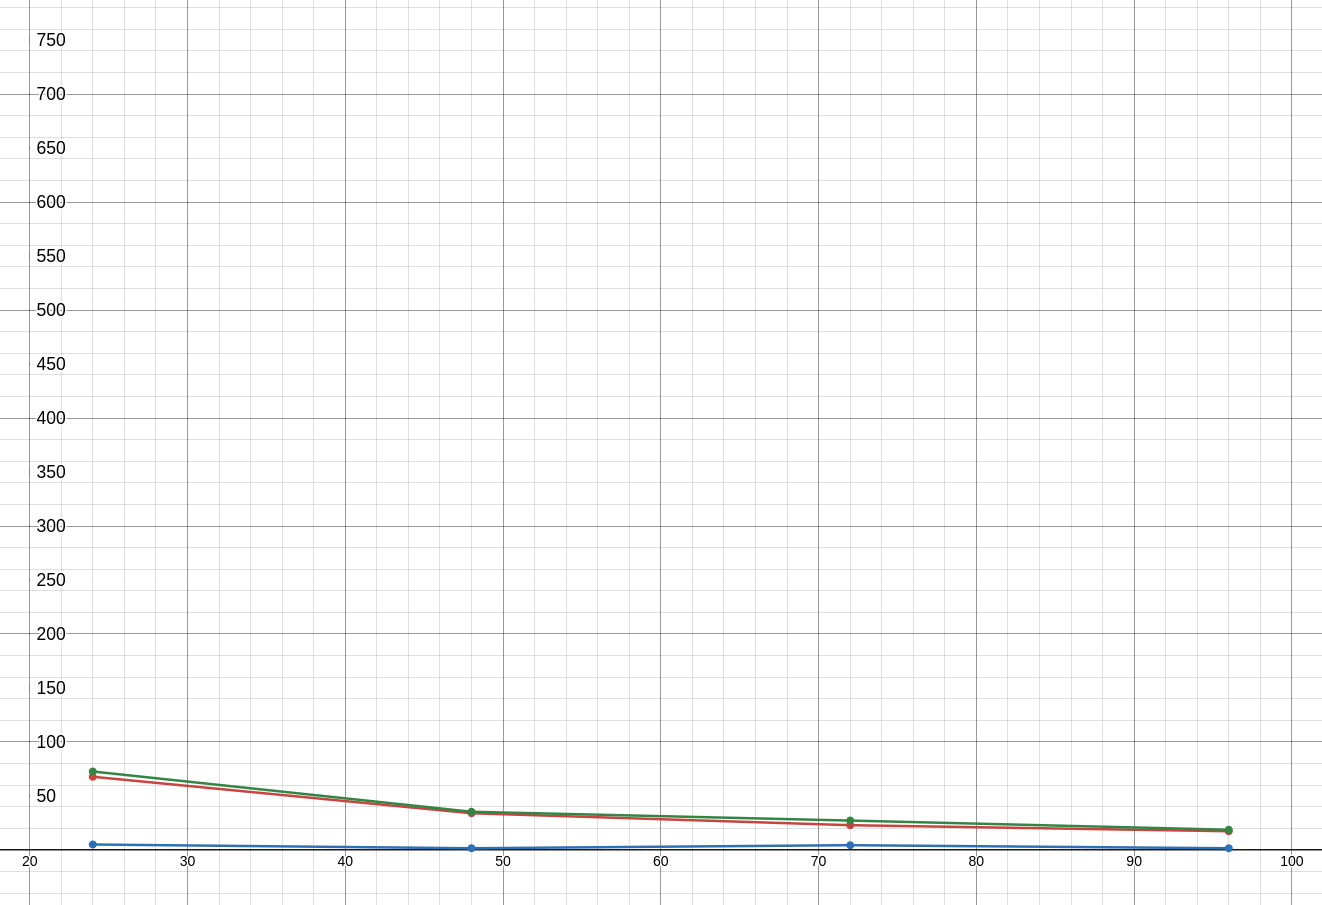
\includegraphics[width=1\linewidth]{graphs/1_kilo.png}
    \caption{Kilo}
  \end{figure}

  \begin{figure}[h]
    \centering
    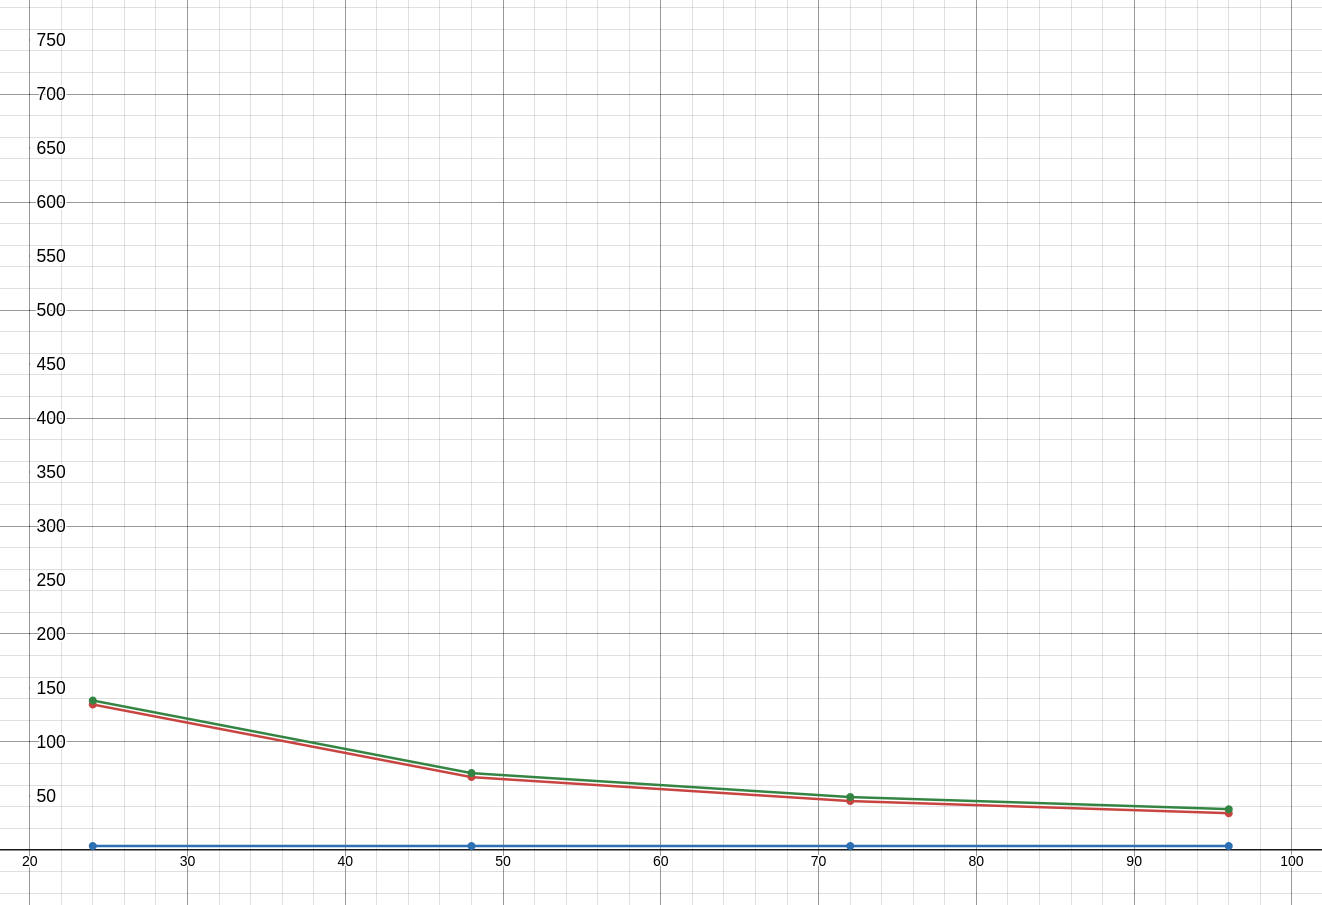
\includegraphics[width=1\linewidth]{graphs/2_mega.png}
    \caption{Mega}
  \end{figure}

  \begin{figure}[h]
    \centering
    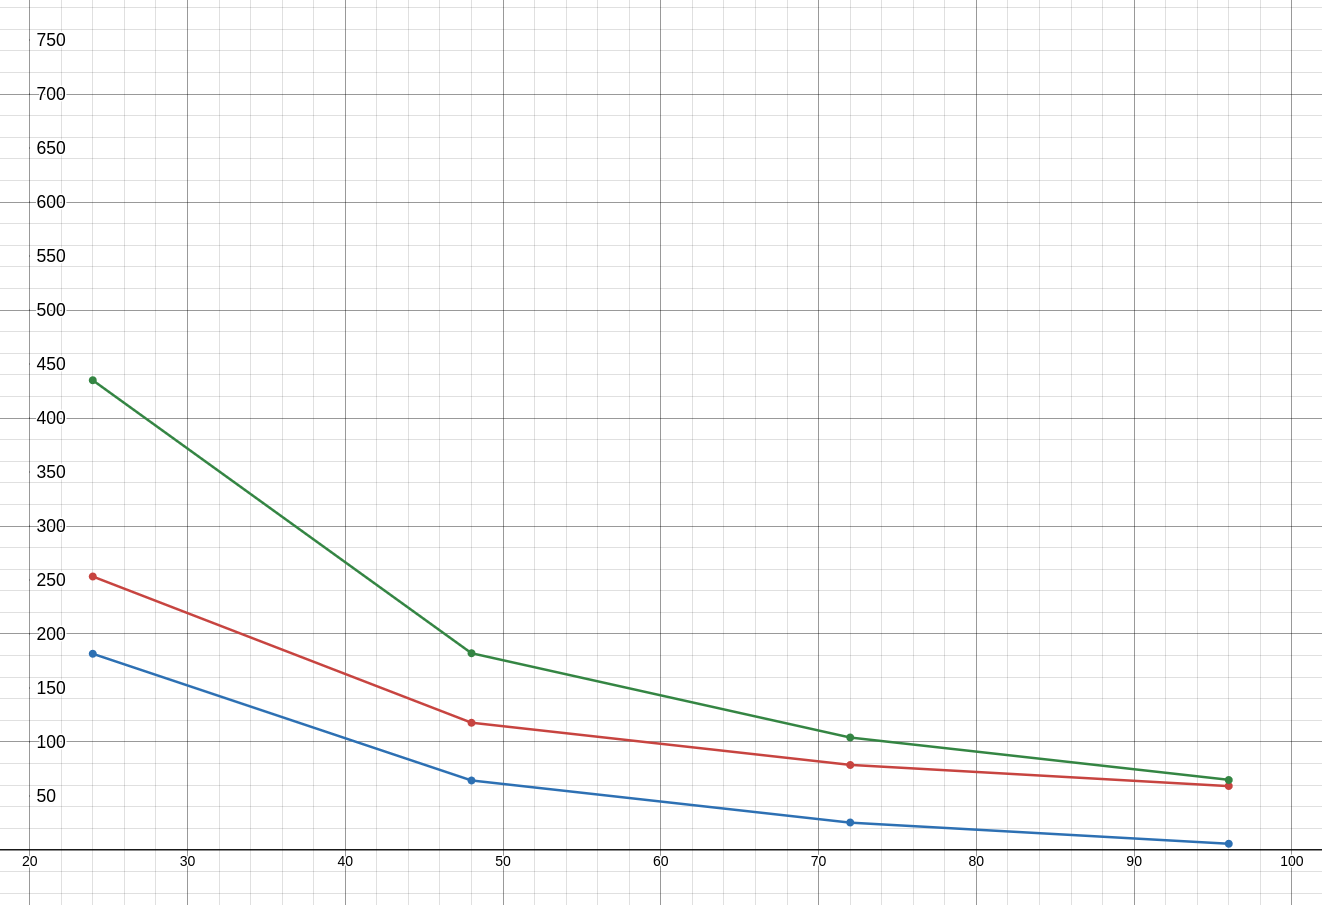
\includegraphics[width=1\linewidth]{graphs/3_giga.png}
    \caption{Giga}
  \end{figure}

  \begin{figure}[h]
    \centering
    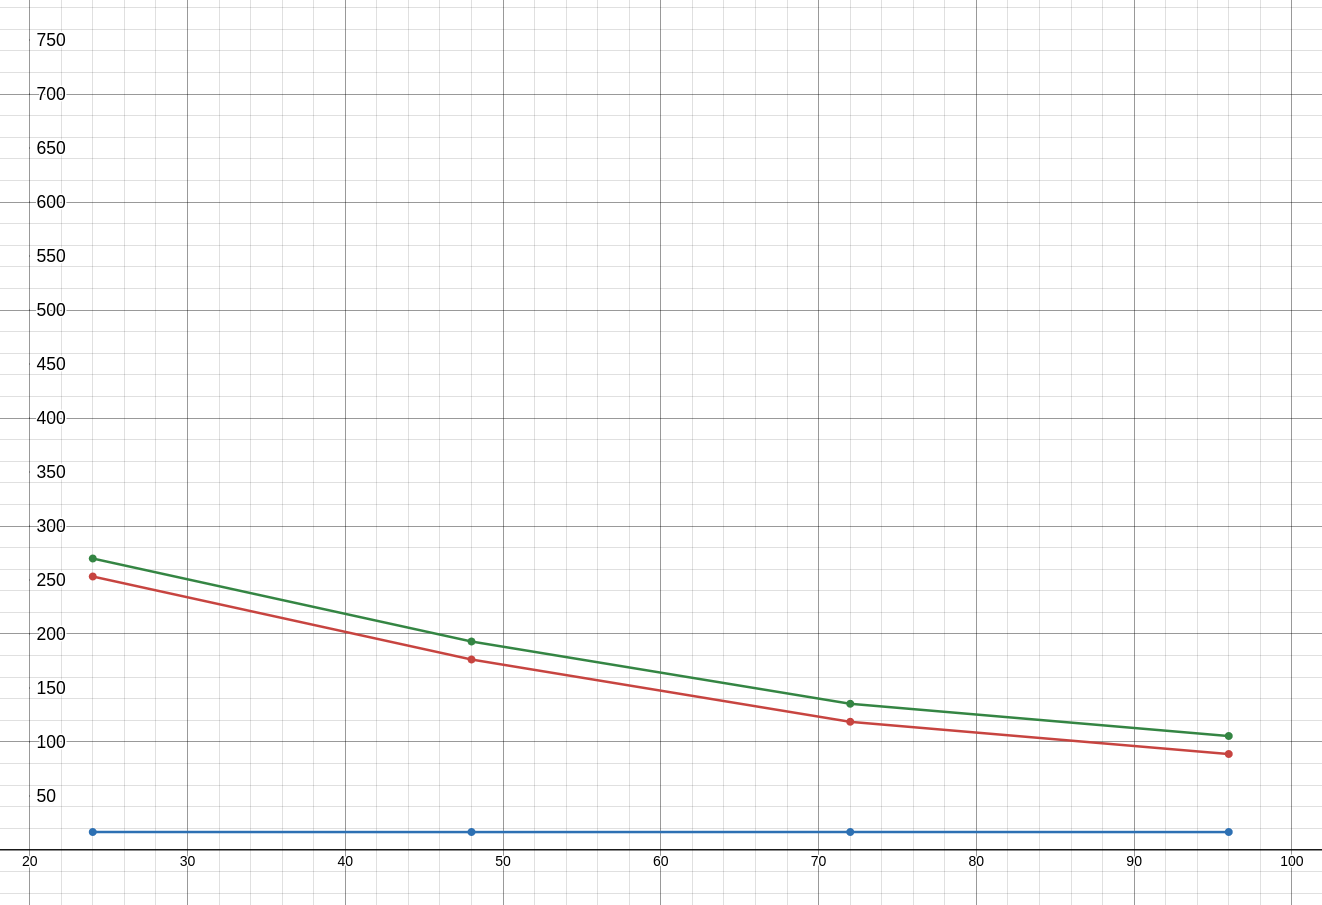
\includegraphics[width=1\linewidth]{graphs/4_tera.png}
    \caption{Tera}
  \end{figure}

  \begin{figure}[h]
    \centering
    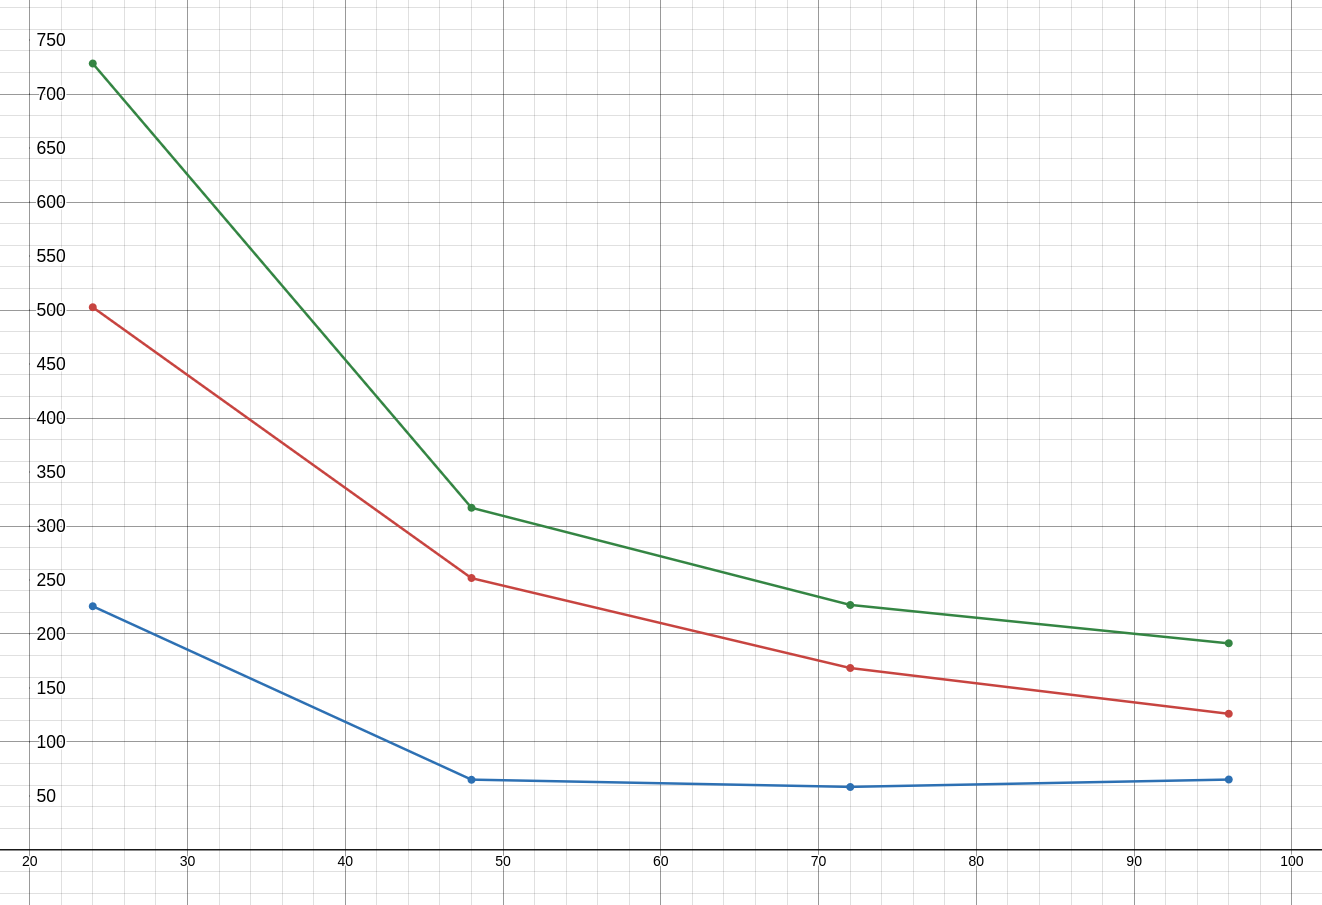
\includegraphics[width=1\linewidth]{graphs/5_peta.png}
    \caption{Peta}
  \end{figure}

  \begin{figure}[h]
    \centering
    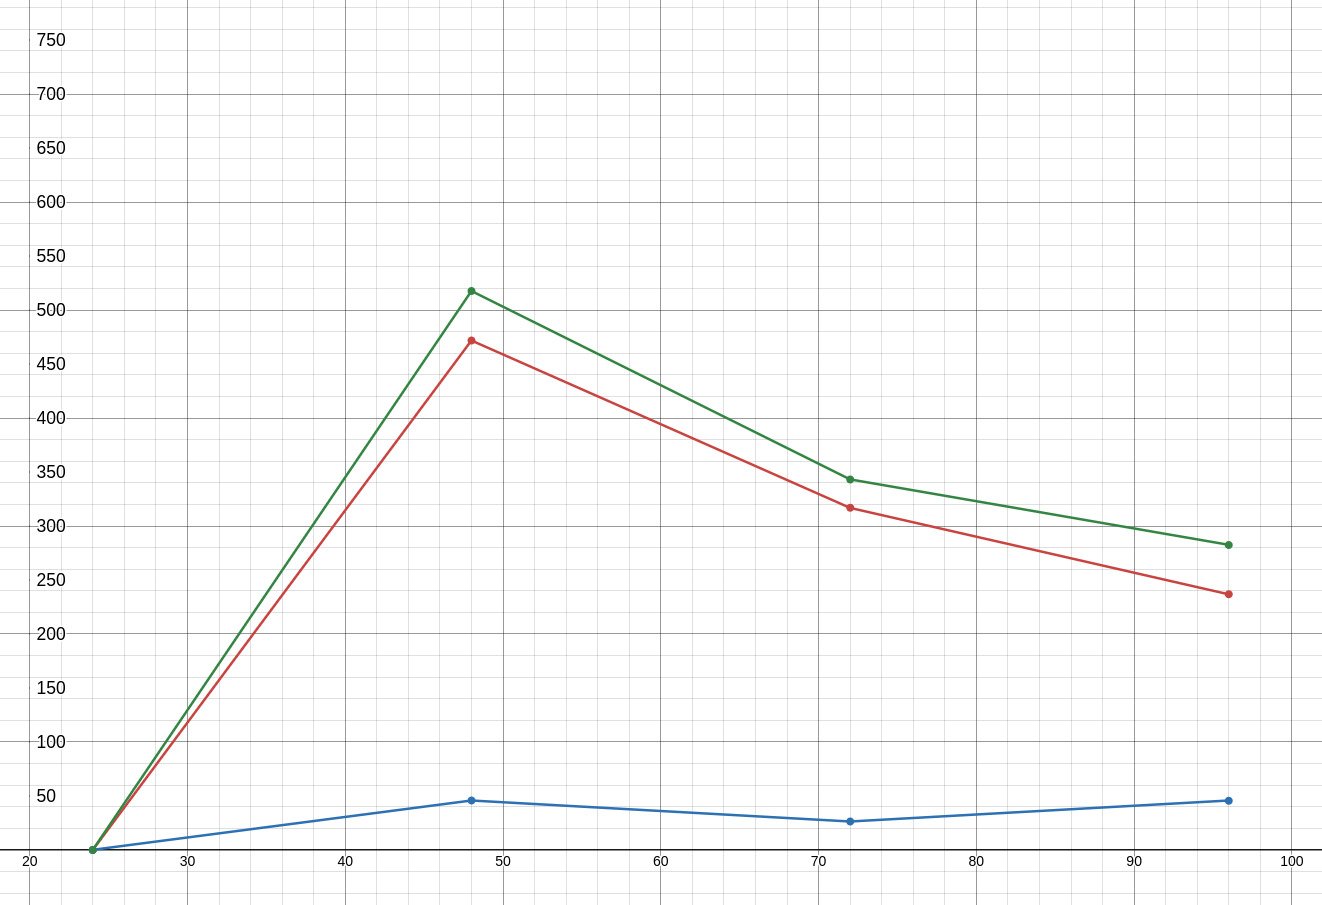
\includegraphics[width=1\linewidth]{graphs/6_exa.png}
    \caption{Exa}
  \end{figure}

\end{document}
